\hypertarget{differential-kinematics}{%
\section{Differential Kinematics}\label{differential-kinematics}}

The last chapter focused on the forward and inverse position kinematics.
There were several problems we had not completely resolved. We want to
address forward and inverse velocity kinematics. This means find
formulas for the end-effector velocities and joint velocities. We also
want to develop some methods to numerically compute the inverse
kinematics. All of these issues can be addressed once we know how to
compute the derivative of the forward kinematics.

\hypertarget{jacobians}{%
\subsection{The Jacobian}\label{jacobians}}

To get started, we will assume that we have the forward kinematic
equations for position in analytic form. Later we can remove this
restriction. For the moment, set aside the DH formalism from the last
section and assume that you have extracted the analytic formulas (or
derived them by some other means). Thus we have the position of the
end-effector as a function of parameters (set of joint values):

\[p = f(q)\]

where \(p\) is the position vector and \(q\) is the joint configuration.
The velocity of the end-effector is given by \(dp/dt\), the time
derivative of position. Since \(f(q)\) is a vector valued function, the
derivative of \(f\) is the time derivative of each component of \(f\):

\[\begin{aligned}
\frac{dp}{dt} =  \begin{pmatrix} \displaystyle \frac{dp_x}{dt} \\[3mm] \displaystyle \frac{dp_y}{dt}  \\[3mm] \displaystyle \frac{dp_z}{dt}  \end{pmatrix}
= \begin{pmatrix} \displaystyle \frac{df_1(q)}{dt} \\[3mm] \displaystyle \frac{df_2(q)}{dt}  \\[3mm] \displaystyle \frac{df_3(q)}{dt}  \end{pmatrix}
= \begin{pmatrix} \displaystyle \nabla f_1 \cdot\frac{dq}{dt} \\[3mm] \displaystyle \nabla f_2\cdot\frac{dq}{dt}  \\[3mm] \displaystyle \nabla f_3 \cdot\frac{dq}{dt}  \end{pmatrix}
= \begin{pmatrix} \displaystyle \nabla f_1 \\[3mm] \displaystyle \nabla f_2  \\[3mm] \displaystyle \nabla f_3  \end{pmatrix} \frac{dq}{dt}
  \equiv J_f \frac{dq}{dt}
\end{aligned}\]

The term \(J_f\) is called the Jacobian and written out, it appears as

\[\begin{aligned}
J_f = \begin{pmatrix}  \frac{\partial f_1} {\partial q_1} & \frac{\partial f_1} {\partial q_2} & \dots & \frac{\partial f_1} {\partial q_m} \\[3mm]
 \frac{\partial f_2} {\partial q_1} & \frac{\partial f_2} {\partial q_2} & \dots & \frac{\partial f_2} {\partial q_m} \\[3mm]
 \frac{\partial f_3} {\partial q_1} & \frac{\partial f_3} {\partial q_2} & \dots & \frac{\partial f_3} {\partial q_m} \end{pmatrix}
\end{aligned}\]

Note that the version above is specific to \(f \in {\Bbb R}^3\) but in
general works for any number of dependent and independent variables.
There will be examples later in the text where we have more than three
dependent variables but for our purposes here, two or three will be
sufficient.

\hypertarget{two-and-three-link-example}{%
\subsubsection{Two and Three link
example}\label{two-and-three-link-example}}

The two and three link manipulators are good examples. The two link
equations are

\[\begin{aligned}
\begin{matrix}
p_x = f_1 = a_2\cos (\theta_1+\theta_2) + a_1 \cos \theta_1 \\
p_y = f_2 = a_2 \sin (\theta_1 +\theta_2) + a_1\sin \theta_1
\end{matrix}
\end{aligned}\]

and the Jacobian of the position equations is

\[\begin{aligned}
J_f = \begin{pmatrix}  \frac{\partial f_1} {\partial q_1} & \frac{\partial f_1} {\partial q_2}  \\[2mm]
 \frac{\partial f_2} {\partial q_1} & \frac{\partial f_2} {\partial q_2}  \end{pmatrix}
 = \begin{pmatrix}  -a_2\sin(\theta_1+\theta_2) - a_1\sin(\theta_1) & -a_2\sin(\theta_1+\theta_2)  \\[2mm]
  a_2\cos (\theta_1+\theta_2) + a_1 \cos (\theta_1) & a_2\cos (\theta_1+\theta_2)  \end{pmatrix}
\end{aligned}\]

where \(q_1 = \theta_1\) and \(q_2 = \theta_2\).

The three link is given by

\[\begin{aligned}
\begin{matrix}
p_x = f_1 = a_3\cos(\theta_1 + \theta_2 + \theta_3)+ a_2 \cos(\theta_1 + \theta_2) + a_1 \cos(\theta_1)\\
p_y = f_2 = a_3\sin(\theta_1 + \theta_2 + \theta_3)+ a_2 \sin(\theta_1 + \theta_2) + a_1 \sin(\theta_1)
\end{matrix}
\end{aligned}\]

and the Jacobian of position is

\[\begin{aligned}
J_f = \begin{pmatrix}  \frac{\partial f_1} {\partial q_1} & \frac{\partial f_1} {\partial q_2} & \frac{\partial f_1} {\partial q_3} \\[2mm]
 \frac{\partial f_2} {\partial q_1} & \frac{\partial f_2} {\partial q_2} & \frac{\partial f_2} {\partial q_3}  \end{pmatrix}
\end{aligned}\]

\[\begin{aligned}
=\begin{pmatrix}  -a_3\sin(\theta_1 + \theta_2 + \theta_3)- a_2 \sin(\theta_1 + \theta_2) - a_1 \sin(\theta_1) & -a_3\sin(\theta_1 + \theta_2 + \theta_3)- a_2 \sin(\theta_1 + \theta_2)  & -a_3\sin(\theta_1 + \theta_2 + \theta_3) \\[2mm]
 a_3\cos(\theta_1 + \theta_2 + \theta_3)+ a_2 \cos(\theta_1 + \theta_2) + a_1 \cos(\theta_1) & a_3\cos(\theta_1 + \theta_2 + \theta_3)+ a_2 \cos(\theta_1 + \theta_2)  & a_3\cos(\theta_1 + \theta_2 + \theta_3)  \end{pmatrix}
\end{aligned}\]

with the obvious choice on \(q_k\).

Compute the Jacobian for the two link manipulator where
\(\theta_1 = 10^\circ, \theta_2 = 20^\circ\).

\hypertarget{listjacobian}{%
\label{listjacobian}}%
\begin{Shaded}
\begin{Highlighting}[]
\NormalTok{θ}\FloatTok{1} \OperatorTok{=} \FloatTok{10}\OperatorTok{*}\NormalTok{π}\OperatorTok{/}\FloatTok{180}
\NormalTok{θ}\FloatTok{2} \OperatorTok{=} \FloatTok{20}\OperatorTok{*}\NormalTok{π}\OperatorTok{/}\FloatTok{180}
\NormalTok{a1 }\OperatorTok{=}\NormalTok{ a2 }\OperatorTok{=} \FloatTok{10}
\NormalTok{j11 }\OperatorTok{=} \OperatorTok{{-}}\NormalTok{a2}\OperatorTok{*}\NormalTok{sin(θ}\FloatTok{1}\OperatorTok{+}\NormalTok{θ}\FloatTok{2}\NormalTok{) }\OperatorTok{{-}}\NormalTok{ a1}\OperatorTok{*}\NormalTok{sin(θ}\FloatTok{1}\NormalTok{)}
\NormalTok{j12 }\OperatorTok{=} \OperatorTok{{-}}\NormalTok{a2}\OperatorTok{*}\NormalTok{sin(θ}\FloatTok{1}\OperatorTok{+}\NormalTok{θ}\FloatTok{2}\NormalTok{)}
\NormalTok{j21 }\OperatorTok{=}\NormalTok{ a2}\OperatorTok{*}\NormalTok{cos(θ}\FloatTok{1}\OperatorTok{+}\NormalTok{θ}\FloatTok{2}\NormalTok{) }\OperatorTok{+}\NormalTok{ a1}\OperatorTok{*}\NormalTok{cos(θ}\FloatTok{1}\NormalTok{)}
\NormalTok{j22 }\OperatorTok{=}\NormalTok{ a2}\OperatorTok{*}\NormalTok{cos(θ}\FloatTok{1}\OperatorTok{+}\NormalTok{θ}\FloatTok{2}\NormalTok{)}
\NormalTok{J }\OperatorTok{=}\NormalTok{ [ j11 j12 }\OperatorTok{;}\NormalTok{ j21 j22]}
\NormalTok{print(J)}
\end{Highlighting}
\end{Shaded}

\hypertarget{jacobianvelocity}{%
\subsection{Velocity}\label{jacobianvelocity}}

Linear velocity is given by \(v = dp/dt\). The joint velocities are
represented by \(\dot{q}\). Returning to the general formula

\[\displaystyle v = \frac{dp}{dt} = J_f \frac{dq}{dt} = J_f \dot{q}\]

This is the forward velocity kinematics. Given the joint velocity
vector, \(\dot{q}\), we can compute the velocity vector, \(v\), by
matrix vector multiplication \(J_f \dot{q}\). Angular velocities should
be converted to radians per unit time.

Example: assume that you have the two link manipulator and given angles
\(\theta_1 = 10^\circ, \theta_2 = 20^\circ\) and angular velocities
\(d\theta_1 / dt = 20^\circ s^{-1}, d\theta_2 / dt = 45^\circ s^{-1}\)
First, convert to radians:
\(d\theta_1 / dt = 20\pi/180 s^{-1}, d\theta_2 / dt = 45\pi/180 s^{-1}\).
Then multiply the Jacobian and the angular velocity vector:

\[\begin{aligned}
J\dot{q} = \begin{pmatrix}  -a_2\sin(\theta_1+\theta_2) - a_1\sin(\theta_1) & -a_2\sin(\theta_1+\theta_2)  \\[2mm]
  a_2\cos (\theta_1+\theta_2) + a_1 \cos (\theta_1) & a_2\cos (\theta_1+\theta_2)  \end{pmatrix}
  \begin{pmatrix} d\theta_1/dt \\ d\theta_2 /dt\end{pmatrix}
  =
   \begin{pmatrix} -6.73648 & -5.0 \\  18.5083  &  8.66025 \end{pmatrix}
    \begin{pmatrix} 20\pi/180 \\ 45\pi/180 \end{pmatrix}
    =  \begin{pmatrix}  -6.866335492 \\  14.87753073867 \end{pmatrix}
\end{aligned}\]

\hypertarget{listvelocity}{%
\label{listvelocity}}%
\begin{Shaded}
\begin{Highlighting}[]
\NormalTok{θ}\FloatTok{1} \OperatorTok{=} \FloatTok{10}\OperatorTok{*}\NormalTok{π}\OperatorTok{/}\FloatTok{180}
\NormalTok{θ}\FloatTok{2} \OperatorTok{=} \FloatTok{20}\OperatorTok{*}\NormalTok{π}\OperatorTok{/}\FloatTok{180}
\NormalTok{a1 }\OperatorTok{=}\NormalTok{ a2 }\OperatorTok{=} \FloatTok{10}
\NormalTok{j11 }\OperatorTok{=} \OperatorTok{{-}}\NormalTok{a2}\OperatorTok{*}\NormalTok{sin(θ}\FloatTok{1}\OperatorTok{+}\NormalTok{θ}\FloatTok{2}\NormalTok{) }\OperatorTok{{-}}\NormalTok{ a1}\OperatorTok{*}\NormalTok{sin(θ}\FloatTok{1}\NormalTok{)}
\NormalTok{j12 }\OperatorTok{=} \OperatorTok{{-}}\NormalTok{a2}\OperatorTok{*}\NormalTok{sin(θ}\FloatTok{1}\OperatorTok{+}\NormalTok{θ}\FloatTok{2}\NormalTok{)}
\NormalTok{j21 }\OperatorTok{=}\NormalTok{ a2}\OperatorTok{*}\NormalTok{cos(θ}\FloatTok{1}\OperatorTok{+}\NormalTok{θ}\FloatTok{2}\NormalTok{) }\OperatorTok{+}\NormalTok{ a1}\OperatorTok{*}\NormalTok{cos(θ}\FloatTok{1}\NormalTok{)}
\NormalTok{j22 }\OperatorTok{=}\NormalTok{ a2}\OperatorTok{*}\NormalTok{cos(θ}\FloatTok{1}\OperatorTok{+}\NormalTok{θ}\FloatTok{2}\NormalTok{)}
\NormalTok{J }\OperatorTok{=}\NormalTok{ [ j11 j12 }\OperatorTok{;}\NormalTok{ j21 j22]}
\NormalTok{qd }\OperatorTok{=}\NormalTok{ [}\FloatTok{25}\OperatorTok{*}\NormalTok{π}\OperatorTok{/}\FloatTok{180} \OperatorTok{;} \FloatTok{45}\OperatorTok{*}\NormalTok{π}\OperatorTok{/}\FloatTok{180}\NormalTok{]}
\NormalTok{J}\OperatorTok{*}\NormalTok{qd}
\end{Highlighting}
\end{Shaded}

\hypertarget{two-and-three-link-example-continued}{%
\subsubsection{Two and three link example
continued}\label{two-and-three-link-example-continued}}

Again we can use the two and three link manipulators as examples. We
first examine the invertability of the two link manipulator Jacobian. A
quick test is to find the determinant. Recall when the determinant is
non-zero, the matrix is invertable. So we have,

\[\begin{aligned}
det(J_f)     = \begin{vmatrix}  -a_2\sin(\theta_1+\theta_2) - a_1\sin(\theta_1) & -a_2\sin(\theta_1+\theta_2)  \\[2mm]
  a_2\cos (\theta_1+\theta_2) + a_1 \cos (\theta_1) & a_2\cos (\theta_1+\theta_2)  \end{vmatrix}
\end{aligned}\]

\[= -a_2^2 \sin(\theta_1+\theta_2)\cos (\theta_1+\theta_2)  - a_1a_2 \sin(\theta_1)\cos (\theta_1+\theta_2) + a_2^2\sin(\theta_1+\theta_2)\cos (\theta_1+\theta_2)
+ a_1a_2 \sin(\theta_1+\theta_2) \cos (\theta_1)\]

\[= a_1a_2 \sin(\theta_2)\]

which implies that this Jacobian is invertable when
\(\theta_2 \neq n\pi\). When \(\theta_2 = n\pi\) then the Jacobian is
rank 1. For the three-link manipulator, the Jacobian is a 2x3 matrix and
as such is not invertable. Since many robot arms have more degrees of
freedom than the dimension of the workspace, can we extract joint
velocity from velocity? For our needs, yes, we will be able to compute
joint velocities using some standard tools from linear algebra. Before
this, we look at the issue of end effector orientation and angular
velocity.

\hypertarget{orientation-and-angular-velocity}{%
\subsubsection{Orientation and angular
velocity}\label{orientation-and-angular-velocity}}

Using the DH derivation, we can determine the end-effector orientation
in addition to position. Recall that we can extract the tool tip
direction from the vector \(\vec{a}\) directly from the DH
transformation \(A\). For the moment, assume that you have an analytic
expression for the orientation vector (Euler angle vector) for the tool
tip: \(\phi\). We can compute the time rate of change of \(\phi\).

\[\dot{\phi} =  J_\phi \dot{q}\]

However, this is not angular velocity in the traditional sense. Angular
velocity, \(\omega\) is the rotation rates in the global or base frame
where \(\dot{\phi}\) gives information in a non-orthogonal sense related
to the end-effector frame. The former being a more intuitive notion of
rotational velocity. It is possible to relate \(\dot{\phi}\) to
\(\omega\), we direct the reader to \texttt{siciliano2009robotics}

\hypertarget{numerical-inverse-kinematics}{%
\subsection{Numerical Inverse
Kinematics}\label{numerical-inverse-kinematics}}

In this section we will look at numerical approaches to the inverse
kinematics problem. First we will assume that the Jacobian is invertable
and second we have a path that we want the end effector to travel. In
addition we are going to restrict our focus on the position kinematics.

Recall the velocity function

\[\displaystyle v = \frac{dp}{dt} = J_f \frac{dq}{dt} = J_f \dot{q}\]

we can invert and gain

\[\displaystyle \dot{q}  = J_f^{-1} v\]

A path in the workspace is represented by \(<x(t),y(t),z(t)>\). You can
compute the derivative of this path
\(v = <\dot{x}(t),\dot{y}(t),\dot{z}(t)>\) . This can be plugged into
the velocity function. Analytically, one can recover the IK via
integration

\[q(t) = \int_0^t J_f^{-1} v(s)ds\]

The path \(<x(t),y(t),z(t)>\) can be known from precise engineering
design or it might be induced from cubic interpolation based on a
sequence of way points from a path plannig algorithm. In practice, the
antiderivative may not be available. And discrete methods are needed.
Discrete methods can focus on discretization of the integration, or
backing up a step and solving the velocity equation in a direct manner.

Assume that you are at a location in space \(<x_0,y_0,z_0>\) and want to
get to \(<x_1,y_1,z_1>\) . The displacement vector, \emph{v} can be used
to find the estimate of \(\dot{q}\).

\[\Delta q = J_f^{-1}v, \quad \mbox{where} \quad v = <x_1-x_0, y_1-y_0, z_1-z_0>\]

We can update \emph{q} via \(q_k = q_{k-1} + \Delta q\). This is a type
of Euler integration (similar to a trapezoid method for integration). It
has discretization error and so after moving the manipulator over the
\(\Delta q\) step, the end effector will not normmally be at
\(<x_1,y_1,z_1>\). Using smaller steps on \emph{v} can help with
accuracy. Using the current point and the old target point, an updated
\emph{v} may be used to correct the step.

A benefit here is that this approach is the basis for a purely numerical
method for inverting the kinematics. The inversion algorithm is

\begin{verbatim}
Input desired target:  p*
Set q values to intial guess (random)
Set stepsize: step

p = FK(q)
d = distance(p, p*)

while d > error
    find v = (p* - p)/||(p* - p)||
    set u = step*v
    find w = inv(J) * u
    set q = q + w
    p = FK(q)
    d = distance(p,p*)
print("q = ", q)
\end{verbatim}

Note that much more sophisticated algorithms exist. Variations of
Newton's Method can be employed here which we will leave to textbooks on
Numerical Methods.

\hypertarget{example}{%
\subsubsection{Example}\label{example}}

In this example we show how one can find the inverse kinematics
numerically for the two link example. Since we have the analytic
formula, we can check our answer. Find \(\theta_1\), \(\theta_2\) when
x=10, y=12 for the two link manipulator when \(a_1=a_2=10\)

\hypertarget{lstnumericaltwolinkik}{%
\label{lstnumericaltwolinkik}}%
\begin{Shaded}
\begin{Highlighting}[]
\KeywordTok{function}\NormalTok{ FK(θ}\FloatTok{1}\OperatorTok{,}\NormalTok{ θ}\FloatTok{2}\OperatorTok{,}\NormalTok{ a1}\OperatorTok{,}\NormalTok{ a2)}
\NormalTok{    x }\OperatorTok{=}\NormalTok{ a2}\OperatorTok{*}\NormalTok{cos(θ}\FloatTok{1}\OperatorTok{+}\NormalTok{θ}\FloatTok{2}\NormalTok{) }\OperatorTok{+}\NormalTok{ a1}\OperatorTok{*}\NormalTok{cos(θ}\FloatTok{1}\NormalTok{)}
\NormalTok{    y }\OperatorTok{=}\NormalTok{ a2}\OperatorTok{*}\NormalTok{sin(θ}\FloatTok{1}\OperatorTok{+}\NormalTok{θ}\FloatTok{2}\NormalTok{) }\OperatorTok{+}\NormalTok{ a1}\OperatorTok{*}\NormalTok{sin(θ}\FloatTok{1}\NormalTok{)}
    \KeywordTok{return}\NormalTok{ x}\OperatorTok{,}\NormalTok{y}
\KeywordTok{end}


\KeywordTok{function}\NormalTok{ FKJ(θ}\FloatTok{1}\OperatorTok{,}\NormalTok{ θ}\FloatTok{2}\OperatorTok{,}\NormalTok{ a1}\OperatorTok{,}\NormalTok{ a2)}
\NormalTok{    j11 }\OperatorTok{=} \OperatorTok{{-}}\NormalTok{a2}\OperatorTok{*}\NormalTok{sin(θ}\FloatTok{1}\OperatorTok{+}\NormalTok{θ}\FloatTok{2}\NormalTok{) }\OperatorTok{{-}}\NormalTok{ a1}\OperatorTok{*}\NormalTok{sin(θ}\FloatTok{1}\NormalTok{)}
\NormalTok{    j12 }\OperatorTok{=} \OperatorTok{{-}}\NormalTok{a2}\OperatorTok{*}\NormalTok{sin(θ}\FloatTok{1}\OperatorTok{+}\NormalTok{θ}\FloatTok{2}\NormalTok{)}
\NormalTok{    j21 }\OperatorTok{=}\NormalTok{ a2}\OperatorTok{*}\NormalTok{cos(θ}\FloatTok{1}\OperatorTok{+}\NormalTok{θ}\FloatTok{2}\NormalTok{) }\OperatorTok{+}\NormalTok{ a1}\OperatorTok{*}\NormalTok{cos(θ}\FloatTok{1}\NormalTok{)}
\NormalTok{    j22 }\OperatorTok{=}\NormalTok{ a2}\OperatorTok{*}\NormalTok{cos(θ}\FloatTok{1}\OperatorTok{+}\NormalTok{θ}\FloatTok{2}\NormalTok{)}
\NormalTok{    J }\OperatorTok{=}\NormalTok{ [ j11 j12 }\OperatorTok{;}\NormalTok{ j21 j22]}
    \KeywordTok{return}\NormalTok{ J}
\KeywordTok{end}

\KeywordTok{function}\NormalTok{ distance(x1}\OperatorTok{,}\NormalTok{ y1}\OperatorTok{,}\NormalTok{ x2}\OperatorTok{,}\NormalTok{ y2)}
\NormalTok{    d }\OperatorTok{=}\NormalTok{ sqrt((x1}\OperatorTok{{-}}\NormalTok{x2)}\OperatorTok{\^{}}\FloatTok{2} \OperatorTok{+}\NormalTok{ (y1}\OperatorTok{{-}}\NormalTok{y2)}\OperatorTok{\^{}}\FloatTok{2}\NormalTok{)}
    \KeywordTok{return}\NormalTok{ d}
\KeywordTok{end}

\KeywordTok{function}\NormalTok{ size(v1}\OperatorTok{,}\NormalTok{v2)}
\NormalTok{    size }\OperatorTok{=}\NormalTok{ sqrt(v1}\OperatorTok{*}\NormalTok{v1}\OperatorTok{+}\NormalTok{v2}\OperatorTok{*}\NormalTok{v2)}
    \KeywordTok{return}\NormalTok{ size}
\KeywordTok{end}

\NormalTok{x }\OperatorTok{=} \FloatTok{10}
\NormalTok{y }\OperatorTok{=} \FloatTok{12}
\NormalTok{θ}\FloatTok{1} \OperatorTok{=} \FloatTok{.1}
\NormalTok{θ}\FloatTok{2} \OperatorTok{=} \FloatTok{.2}
\NormalTok{a1 }\OperatorTok{=}\NormalTok{ a2 }\OperatorTok{=} \FloatTok{10}
\NormalTok{step }\OperatorTok{=} \FloatTok{0.1}
\NormalTok{xc}\OperatorTok{,}\NormalTok{ yc }\OperatorTok{=}\NormalTok{ FK(θ}\FloatTok{1}\OperatorTok{,}\NormalTok{ θ}\FloatTok{2}\OperatorTok{,}\NormalTok{ a1}\OperatorTok{,}\NormalTok{ a2)}
\NormalTok{d }\OperatorTok{=}\NormalTok{ distance(x}\OperatorTok{,}\NormalTok{y}\OperatorTok{,}\NormalTok{xc}\OperatorTok{,}\NormalTok{yc)}

\KeywordTok{while}\NormalTok{ d }\OperatorTok{\textgreater{}} \FloatTok{.01}
\NormalTok{    vx }\OperatorTok{=}\NormalTok{ x }\OperatorTok{{-}}\NormalTok{ xc}
\NormalTok{    vy }\OperatorTok{=}\NormalTok{ y }\OperatorTok{{-}}\NormalTok{ yc}
\NormalTok{    s }\OperatorTok{=}\NormalTok{ size(vx}\OperatorTok{,}\NormalTok{vy)}
\NormalTok{    ux }\OperatorTok{=}\NormalTok{ step}\OperatorTok{*}\NormalTok{vx}\OperatorTok{/}\NormalTok{s}
\NormalTok{    uy }\OperatorTok{=}\NormalTok{ step}\OperatorTok{*}\NormalTok{vy}\OperatorTok{/}\NormalTok{s}
\NormalTok{    J }\OperatorTok{=}\NormalTok{ FKJ(θ}\FloatTok{1}\OperatorTok{,}\NormalTok{ θ}\FloatTok{2}\OperatorTok{,}\NormalTok{ a1}\OperatorTok{,}\NormalTok{ a2)}
\NormalTok{    u }\OperatorTok{=}\NormalTok{ [ux}\OperatorTok{,}\NormalTok{ uy]}
\NormalTok{    w }\OperatorTok{=}\NormalTok{ J}\OperatorTok{\textbackslash{}}\NormalTok{u}
\NormalTok{    θ}\FloatTok{1} \OperatorTok{=}\NormalTok{ θ}\FloatTok{1} \OperatorTok{+}\NormalTok{ w[}\FloatTok{1}\NormalTok{]}
\NormalTok{    θ}\FloatTok{2} \OperatorTok{=}\NormalTok{ θ}\FloatTok{2} \OperatorTok{+}\NormalTok{ w[}\FloatTok{2}\NormalTok{]}
\NormalTok{    xc}\OperatorTok{,}\NormalTok{ yc }\OperatorTok{=}\NormalTok{ FK(θ}\FloatTok{1}\OperatorTok{,}\NormalTok{ θ}\FloatTok{2}\OperatorTok{,}\NormalTok{ a1}\OperatorTok{,}\NormalTok{ a2)}
\NormalTok{    d }\OperatorTok{=}\NormalTok{ distance(x}\OperatorTok{,}\NormalTok{y}\OperatorTok{,}\NormalTok{xc}\OperatorTok{,}\NormalTok{yc)}
\KeywordTok{end}
\NormalTok{println(}\StringTok{"θ1 = "}\OperatorTok{,}\NormalTok{θ}\FloatTok{1}\OperatorTok{,} \StringTok{"θ2 = "}\OperatorTok{,}\NormalTok{ θ}\FloatTok{2}\OperatorTok{,} \StringTok{"  x = "}\OperatorTok{,}\NormalTok{ xc}\OperatorTok{,} \StringTok{"  y = "}\OperatorTok{,}\NormalTok{ yc)}
\end{Highlighting}
\end{Shaded}

We can use the builtin nonlinear solver in Julia as well:

\hypertarget{lstnumericaltwolinkiknlsolve}{%
\label{lstnumericaltwolinkiknlsolve}}%
\begin{Shaded}
\begin{Highlighting}[]
\CommentTok{\#import Pkg}
\CommentTok{\#Pkg.add("NLsolve")}

\KeywordTok{using}\NormalTok{ NLsolve}

\KeywordTok{function}\NormalTok{ f}\OperatorTok{!}\NormalTok{(F}\OperatorTok{,}\NormalTok{ x)}
\NormalTok{    F[}\FloatTok{1}\NormalTok{] }\OperatorTok{=} \FloatTok{10}\OperatorTok{*}\NormalTok{cos(x[}\FloatTok{1}\NormalTok{]}\OperatorTok{+}\NormalTok{x[}\FloatTok{2}\NormalTok{]) }\OperatorTok{+} \FloatTok{10}\OperatorTok{*}\NormalTok{cos(x[}\FloatTok{1}\NormalTok{]) }\OperatorTok{{-}} \FloatTok{10}
\NormalTok{    F[}\FloatTok{2}\NormalTok{] }\OperatorTok{=} \FloatTok{10}\OperatorTok{*}\NormalTok{sin(x[}\FloatTok{1}\NormalTok{]}\OperatorTok{+}\NormalTok{x[}\FloatTok{2}\NormalTok{]) }\OperatorTok{+} \FloatTok{10}\OperatorTok{*}\NormalTok{sin(x[}\FloatTok{1}\NormalTok{]) }\OperatorTok{{-}} \FloatTok{12}
\KeywordTok{end}


\KeywordTok{function}\NormalTok{ j}\OperatorTok{!}\NormalTok{(J}\OperatorTok{,}\NormalTok{ x)}
\NormalTok{    J[}\FloatTok{1}\OperatorTok{,} \FloatTok{1}\NormalTok{] }\OperatorTok{=} \OperatorTok{{-}}\FloatTok{10}\OperatorTok{*}\NormalTok{sin(x[}\FloatTok{1}\NormalTok{]}\OperatorTok{+}\NormalTok{x[}\FloatTok{2}\NormalTok{]) }\OperatorTok{{-}} \FloatTok{10}\OperatorTok{*}\NormalTok{sin(x[}\FloatTok{1}\NormalTok{])}
\NormalTok{    J[}\FloatTok{1}\OperatorTok{,} \FloatTok{2}\NormalTok{] }\OperatorTok{=} \OperatorTok{{-}}\FloatTok{10}\OperatorTok{*}\NormalTok{sin(x[}\FloatTok{1}\NormalTok{]}\OperatorTok{+}\NormalTok{x[}\FloatTok{2}\NormalTok{])}
\NormalTok{    J[}\FloatTok{2}\OperatorTok{,} \FloatTok{1}\NormalTok{] }\OperatorTok{=} \FloatTok{10}\OperatorTok{*}\NormalTok{cos(x[}\FloatTok{1}\NormalTok{]}\OperatorTok{+}\NormalTok{x[}\FloatTok{2}\NormalTok{]) }\OperatorTok{+} \FloatTok{10}\OperatorTok{*}\NormalTok{cos(x[}\FloatTok{1}\NormalTok{])}
\NormalTok{    J[}\FloatTok{2}\OperatorTok{,} \FloatTok{2}\NormalTok{] }\OperatorTok{=} \FloatTok{10}\OperatorTok{*}\NormalTok{cos(x[}\FloatTok{1}\NormalTok{]}\OperatorTok{+}\NormalTok{x[}\FloatTok{2}\NormalTok{])}
\KeywordTok{end}

\NormalTok{nlsolve(f}\OperatorTok{!,}\NormalTok{ j}\OperatorTok{!,}\NormalTok{ [ }\FloatTok{0.1}\OperatorTok{;} \FloatTok{.2}\NormalTok{])}
\end{Highlighting}
\end{Shaded}

The

Both of these programs will exit with errors if you set the intitial
value to {[}0,0{]}. The Jacobian is singular and so the embedded linear
solve will fail. This is addressed below. First we discuss the approach
to numerically computing the Jacobian.

\hypertarget{numerical-jacobian-1}{%
\subsection{Jacobian numerical approaches}\label{numerical-jacobian-1}}

Using the DH Convention approach, we have the manipulator can be
represented by

\[A = \prod_{i=0}^m A_i\]

Assume for the moment that each \(A_i\) has only on parameter that
varies. One can generalize from this case and it is sufficient here.
This gives us a nice way to compute the Jacobian. We start by computing
a single partial derivative.

\[\displaystyle \frac{\partial A}{\partial q_k} = \displaystyle \frac{\partial}{\partial q_k} \prod_{i=0}^m A_i (q_i)=
\displaystyle A_1(q_1) A_2(q_2) \dots A_{k-1}(q_{k-1}) \frac{\partial A_k}{\partial q_k} A_{k+1}(q_{k+1})\dots A_m (q_m)\]

Define \(\frac{\partial A_k}{\partial q_k} = A_k'\) and we have

\[B_k = A_1A_2 \dots A_k' \dots A_m\]

If we have the row index as \emph{i} and the column index as \emph{j},
we now add the slice index \emph{k}. All of the \(B_k\) can be stacked
into a tensor \(B\).

\begin{figure}
\centering
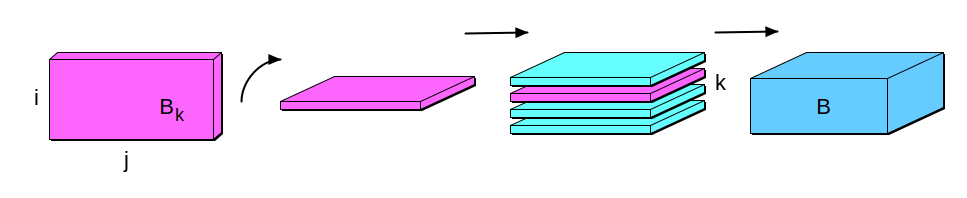
\includegraphics[width=0.75\textwidth,height=\textheight]{SimulationFigures/tensor.*}
\caption{}
\end{figure}

The Jacobian of the position function can be found in this tensor as a
partial slice where \emph{j=4} and for \emph{i=1:3} and all \emph{k}:

\begin{figure}
\centering
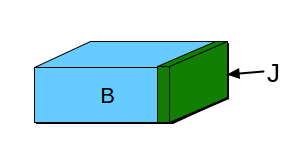
\includegraphics[width=0.25\textwidth,height=\textheight]{SimulationFigures/tensor2.*}
\caption{}
\end{figure}

\hypertarget{invertability-of-the-jacobian}{%
\subsection{Invertability of the
Jacobian}\label{invertability-of-the-jacobian}}

We saw that for the two link manipulator, the Jacobian of the forward
position kinematics was not invertable for a discrete set of parameter
values. For the three link manipulator we saw that the Jacobian FPK was
not square and so not invertable. For the general case, we have an
non-square Jacobian, \(n \times m\):

\[v = J_f \dot{q}\]

We have from earlier that we can find a least squares solution (via
right inverse or the SVD):

\[\dot{q} = J_f^+ v\]

This does work like the case above when the Jacobian is invertable. The
pseudoinverse can move the robot arm in the desired direction. It is
helpful to understand the geometry. Normally this is an underdetermined
system. Generically we are mapping \({\Bbb R}^m \to {\Bbb R}^3\) with
\(m > 3\). The extra dimensions need to be compressed down to fit into
three dimensions. This happens by mapping those dimensions to zero. Let
\(u\) be one of these directions.

\[J_f u = 0\]

u is an element of the Nullspace of \(J_f\). The domain, \({\Bbb R}^m\)
can be partitioned into the row space and the nullspace.

\[x = w + u\]

where \(w\) is in the row space and \(u\) is in the nullspace. Another
terminology is that \emph{w} is the particular solution and \emph{u} is
the homgeneous solution. It is not hard to verify that \(u \perp w\).
Moving joints in the null direction does not move the end-effector but
does reconfigure the robot arm. Moving joints in the rowspace direction
does move the end-effector.

There is one and only one solution to \(v = J_f \dot{q}\) when
\(\dot{q}\) is restricted to the row space. A general solution to the
problem is

\[x_g = w + cu\]

where \emph{c} is any real number. We can address this via the SVD.
Given the matrix \(J_f\) we can factor in the following manner:

\[J_f  = U \Sigma^+ V^*\]

where \(U\) is a \(n \times n\) unitary matrix, \(\Sigma\) is a
\(n \times m\) diagonal matrix, and \(V\) is a \(m \times m\) unitary
matrix. Recall that unitary means \(UU^* = I\) where
\(U^* = \bar{U}^T\), the complex conjugate transpose.

The pseudoinverse will provide the row and nullspace \emph{w} :

\[w = J_f^+ v = V \Sigma^+ U^T v\]

If we used the SVD to compute \(J_f^+\) then we have the nullspace as
well. A basis for the nullspace are the rows of \(V^*\) that correspond
to \textbf{zero} diagonal elements in \(\Sigma\).

\hypertarget{example-1}{%
\subsubsection{Example}\label{example-1}}

We will illustrate these ideas with the three link manipulator.
